% !TEX encoding = UTF-8 Unicode
% !TEX root = ../main.tex
% !TEX spellcheck = en-US



% DEFINITION AND CHALLENGES, HOW IT RELATES TO THIS THESIS

% LINKING WORDS ARE IMPORTANT; similarly, in addition, also, again
% Disagreements; however, on the otehr hand, conversely, nevertheless

% Structure:

% - Introduction/definition of topic

\chapter{State-of-the-Art}
This chapter presents the state-of-the-art topics which are relevant to this thesis. Section 2.1 presents the metaphor of technical debt. 









%%%%%%%%%%%%%%%%%%%%%%%%%%%%%%%%%%%%%%%%%%%%%%% TECHNICAL DEBT %%%%%%%%%%%%%%%%%%%%%%%%%%%%%%%%%%%%%%%%%%%%%%%



\section{Technical Debt}
The metaphor of technical debt was first introduced by Ward Cunningham in 1992 to communicate technical problems with non-technical stakeholders\cite{p29-cunningham}. To deliver business functionality as quick as possible, \textit{'quick and dirty'} decisions are often made. These decisions may have short-term value, but it could affect future development and maintenance activities negatively. Cunningham was the first one who drew the comparison between technical complexity and financial debt in a 1992 experience report\cite{p29-cunningham}: 

\begin{displayquote}
	\textit{“Shipping first time code is like going into debt. A little debt speeds up the development as long as it is paid back promptly with a rewrite... The danger occurs when the debt is not repaid. Every minute spent on not-quite-right code counts as interest on that debt. Entire engineering organizations can be brought to a stand-still under the debt load of an unconsolidated implementation, object-oriented or otherwise.” - Ward Cunningham, 1992}.
\end{displayquote}

The concept refers to the financial world where going into debt means repaying the loan with interest\cite{p50-allman}. Like financial debt, technical debt accrues interest over time. Interest is defined as the extra effort that has to be dedicated in the future development in order to modify the part of the software that contains technical debt\cite{p31-guo,p35-klinger,li2015systematic}. Unmanaged technical debt can cause projects to face significant technical and financial problems, which ultimately leads to increased maintenance and evolution costs\cite{nord2012search}. 



\subsection{Definitions of Technical Debt}
Several researchers have attempted to give us a clear picture of what technical debt is\cite{url-fowler,url-mcconnell,krutchen}. Fowler\cite{url-fowler} presents a technical debt quadrant which consists of two dimensions: \textit{reckless/prudent} and \textit{deliberate/inadvertent}\cite{url-fowler}. Technical debt quadrant in Figure \ref{fig:techDebtQuad} indicates four types of technical debt: \textit{reckless/deliberate}, \textit{reckless/inadvertent}, \textit{prudent/deliberate}, and \textit{prudent/inadvertent}. Reckless/Deliberate debt is usually incurred when technical decisions are taken intentionally without any plans on how to address the problem in the future. A team may know about good design practices, but still implements \textit{'quick and dirty'} solutions because they think they cannot afford the time required to write clean code. The second type is reckless/inadvertent. It is incurred when best practices for code and design are being ignored, ultimately leading to a big mess of spaghetti code. Prudent/Deliberate debt occurs when the value of implementing a ‘quick and dirty’ solution is worth the cost of incurring the debt to meat a short-term goal. The team is fully aware of the consequences, and have a plan on how to address the problem in the future. At last, we have prudent/inadvertent debt. This type of debt occurs when a team realizes that the design of a valuable software could have been better after delivering it. A software development process is much as learning as it is coding.

\begin{figure}[ht!]
	\centering
	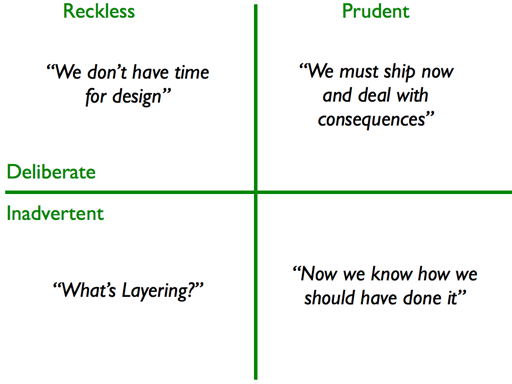
\includegraphics[width=0.8\textwidth]{images/techDebtQuadrant.png}
	\caption{Fowler's Technical Debt Quadrant}
	\label{fig:techDebtQuad}
\end{figure}

McConnell\cite{url-mcconnell} classified technical debt as intentional and unintentional debt. Intentional debt is described as debt that is incurred deliberately. For example, an organization makes a strategic decision that aims to reach a certain objective by taking a shortcut they are fully aware of. Intentional debt can further be viewed as short-term and long-term debt\cite{p8-codabux,mcconnel-slides}. Short-term debt is usually incurred reactively, for tactical reasons. Long-term debt is usually incurred pro-actively, for strategic reasons. Unintentional debt is described as debt that is incurred inadvertently due to lack of knowledge or experience. For example, a junior software developer may write low quality code that does not conform with standard coding standard due to low experience. 

Krutchen et al.\cite{krutchen} presented a technical debt landscape for organizing technical debt. They distinguished visible elements such as new functionality to add or defects to fix, and the invisible elements that are only visible to software developers. On the left side of Figure \ref{fig:techDebtLandscape}, technical debt affects evolvability of the system, while on the right side, technical debt mainly affects software maintainability. 

\begin{figure}[ht!]
	\centering
	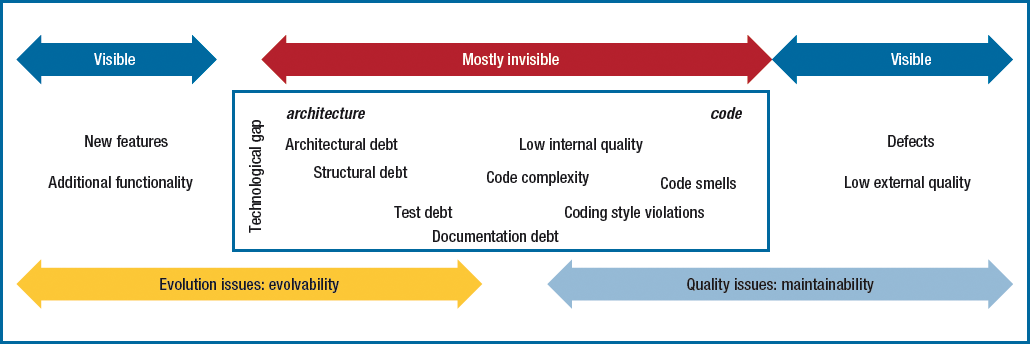
\includegraphics[width=1.0\textwidth]{images/techDebtLandscape.png}
	\caption{Technical Debt Landscape}
	\label{fig:techDebtLandscape}
\end{figure}

\subsection{Classification of Technical Debt}
\label{sub:classificationtechdebt}
Technical debt can accumulate in many different ways, and therefore it is important to distinguish the various types of technical debt. Multiple studies\cite{li2015systematic,p8-codabux,foser076-brown,tom2013exploration,Zazworka:2011:PDD:1985362.1985372,Zazworka:2013:CSE:2460999.2461005} have pointed out several subcategories of technical debt based on its association with traditional software life-cycle phases; architectural debt, code debt, defect debt, design debt, documentation debt, infrastructure debt, requirements debt, and test debt. Table \ref{tab:subcategories} lists the different subcategories of technical debt.

\begin{table}
	\resizebox{\textwidth}{!}{
	\centering
	\begin{tabular}{ | p{5cm} | p{8cm} |}
	\hline
	\textbf{Subcategory} & \textbf{Definition} \\ \hline
	Architectural debt\cite{li2015systematic,p8-codabux,foser076-brown} & Architectural decisions that make compromises in some of the quality attributes, such as modifiability. \\ \hline
	Code debt\cite{li2015systematic,foser076-brown,tom2013exploration} & Poorly written code that violates best coding practices and guidelines, such as code duplication. \\ \hline
	Defect debt\cite{li2015systematic,tom2013exploration} & Defect, failures, or bugs in the software. \\ \hline
	Design debt\cite{li2015systematic,Zazworka:2011:PDD:1985362.1985372,foser076-brown} & Technical shortcuts that are taken in design.\\ \hline
	Documentation debt\cite{li2015systematic,foser076-brown,Zazworka:2013:CSE:2460999.2461005} & Refers to insufficient, incomplete, or outdated documentation in any aspect of software development.\\ \hline
	Infrastructure debt\cite{li2015systematic,tom2013exploration,p8-codabux} & Refers to sub-optimal configuration of development-related processes, technologies, and supporting tools. An example is lack of continuous integration.\\ \hline
	Requirements debt\cite{li2015systematic,Zazworka:2013:CSE:2460999.2461005} & Refers to the requirements that are not fully implemented, or the distance between actual requirements and implemented requirements.\\ \hline
	Test debt\cite{li2015systematic,Zazworka:2013:CSE:2460999.2461005,foser076-brown} & Refers to shortcuts taken in testing. An example is lack of unit tests, and integration tests.\\
	\hline
	\end{tabular}}
	\caption{Types of Technical Debt} \label{tab:subcategories}
\end{table}


\subsection{Causes and Effects of Technical Debt}
Several researchers have investigated the reasons to incur technical debt. Klinger et al.\cite{p35-klinger} conducted an industrial case study at IBM where four technical architects with different backgrounds were interviewed. The goal was to examine how decisions to incur debt were taken, and the extent to which the debt provided leverage\cite{p35-klinger}. The study revealed that the company failed to assess the impact of intentionally incurring debt on projects. Decisions regarding technical debt were rarely quantified. The study also revealed big organizational gaps among the business, operational, and technical stakeholders. When the project team felt pressure from the different stakeholders, technical debt decisions were made without quantifications of possible impacts.

Lim et al.\cite{lim-taksande} pointed out that technical debt is not always the result of poor developer disciplines, or sloppy programming. It can also include intentional decisions to trade off competing concerns during business pressure. Furthermore, Li et al. explains that technical debt can be used in short term to capture market share and to collect customers feedback early. In the long term, technical debt tended to be negative. These trade-offs included increased complexity, reduced performance, low maintainability, and fragile code. This led to bad customer satisfaction and extra working hours. In many cases, the short term benefits of technical debt outweighed the future costs.

Guo et al.\cite{guo2011tracking} studied the effects of technical debt by tracking a single delayed maintenance task in a real software project throughout its life-cycle, and simulated how managing technical debt can impact the project result. The results indicated that delaying the maintenance task would have almost tripled the costs, if it had been done later.

Siebra et al.\cite{p247-siebra} carried out an industrial case study where they analyzed documents, emails, and code files. Additionally, they interviewed multiple developers and project managers. The case study revealed that technical debt were mainly taken by strategic decisions. Furthermore, they commented out that using a unique specialist could lead the development team to solutions that the specialist wanted and believe were correct, leading the team to incur debt. The study also identified that technical debt can both increase and decrease the amount of working hours.

Zazworka et al.\cite{zazworka2011investigating} studied the effects of god classes and technical debt on software quality. God classes are examples on bad coding, and therefore includes a possibility for refactoring\cite{Zazworka:2011:PDD:1985362.1985372}. The results indicated that god classes require more maintenance effort including bug fixing and changes to software that are considered as a cost to software project. In other words, if developers desire higher software quality, then technical debt needs to be addressed closely in the development process.

Buschmann\cite{buschmann2011pay} explained three different stories of technical debt effects. In the first case, technical debt accumulated in a platform started had growth to a point where development, testing, and maintenance costs started to increase dramatically. Additionally, the components were hardly usable. In the second case, developers started to use shortcuts to increase the development speed. This resulted in significant performance issues because an improper software modularization reflected organizational structures instead of the system domains. It ended up turning in to economic consequences. In the last case, an existing software product experienced increased maintenance cost due to architectural erosion. However, management analyzed that re-engineering the whole software would cost more than doing nothing. Management decided not to do anything to technical debt, because it was cheaper from a business point-of-view.

Codabux et al.\cite{p8-codabux} carried out an industrial case study where the topic was agile development focusing on technical debt. They observed and interviewed developers to understand how technical debt is characterized, addressed, prioritized, and how decisions led to technical debt. Two subcategories of technical debt were commonly described in this case study; infrastructure and automation debt. 

These studies indicates that the causes and effects of technical debt are not always caused by technical reasons. Technical debt can be the result of intentional decisions made by the different stakeholders. Incurring technical debt may have short-term positive effects such as time-to-market benefits. Not paying down technical debt can result economic consequences, or quality issues in the long-run. The allowance of technical debt can facilitate product development for a period, but decreases the product maintainability in the long-term. However, there are some times where short-term benefits overweight long-term costs\cite{guo2011tracking}. 


\subsection{Identification of Technical Debt}
Technical debt accumulation may cause increased maintenance and evolution costs. At worst, it may even cancel out projects. The first step towards managing technical debt is to properly identify and visualize  technical debt items. 

According to Zazworka et al.\cite{zazworka2014comparing}, there are four main techniques for identifying technical debt in source code: modularity violations, design patterns and grime buildup, code smells, and automatic static analysis issues. 

\subsubsection{Modularity Violation}
Software modularity determines software quality in terms of evolveability, changeability, and maintainability\cite{huynh2007evolutionary}, and the essence is to allow modules to evolve independently. However, in reality, two software components may change together though belonging to distinct modules, due to unwanted side effects caused by \textit{'quick and dirty'} solutions\cite{wong2011detecting,zazworka2014comparing}. This causes a violation in the software designed modular structure, which is called a modularity violation. Wong et al.\cite{wong2011detecting} identified 231 modularity violations from 490 modification requests in their experiment using Hadoop. 152 of the 490 identified violations were confirmed by the fact that they were either addressed in later versions of Hadoop, or recognized as problems by the developers. In addition, they identified 399 modularity violation from 3458 modification request of Eclipse JDT\cite{wong2011detecting}. Among these violations, 161 were confirmed. Zazworka et al.\cite{zazworka2014comparing} revealed that the average number of modularity violations per class in release 0.2.0 to release 0.14.0 of Hadoop ranged from 0.04 to 0.11. They identified 8 modularity violations in the first release of Hadoop and 37 in the last one. In addition, they revealed that modularity violations are strongly related to classes with high defect- and change-proneness. 



\subsubsection{Design Pattern and Grime Buildup}
Patterns are known to be general solutions to recurrent design problems. They are commonly used to improve maintainability and architecture design of software systems. 23 design patterns are widely used in software development and is classified into three types: creational, behavioural, and structural. What each include.

nevn noen fordeler med bruk av design patterns.


% decay, change, root

However, software continuously evolve in response to external demands for new functionality. One consequence of such evolution is software design decay. Izurieta et al.\cite{izurieta2007software} defines decay the deterioration of the internal structure of system designs. Furthermore, they define Design pattern decay as deterioration of the structural integrity of a design pattern realization. That is, as a pattern realization evolves, its structure and behavior tend to deviate from its original intent. Design pattern grime is a specific type of design pattern decay\cite{izurieta2007software}. 

However, changes in the code base could lead to code ending up outside the pattern. This is known as design grime. 




\subsubsection{Code Smell}
\label{subsub:codesmell}
Some forms of technical debt accumulate over time in the form of source code\cite{zazworka2014comparing}. Fowler et al.\cite{fowler1999refactoring} describes the concept of code smells as choices in object-oriented systems that does not comply with the principles of good object-oriented design and programming practices. They are an indication of that some parts of the design is inappropriate and that it can be improved. Code smells are usually removed by performing one or more refactoring\cite{fowler1999refactoring}. For instance, one such smell is "Long Method", a method with too many lines of code. This type of code smell can be refactored by 'Extract Method', by reducing the length of the method body\cite{fowler1999refactoring}. 

Mäntylä et al.\cite{mantyla2003taxonomy} proposes a taxonomy based on the criteria on code smells defined by Fowler et al.\cite{fowler1999refactoring}. The taxonomy categories code smells into seven groups of problems: bloaters, object-oriented abusers, change preventers, dispensables, encapsulators, couplers, and others. The first class, Bloaters, represents large pieces of code that cannot be effectively handled. Object-oriented abusers is related to cases where the solution does not exploit the the possibilities of object-oriented design. Change preventers refers to code structure that considerably hinder the modification of software. Dispensables represent code structure with no value. Encapsulators deal with data communication mechanism or encapsulation. Couplers refers to classes with high coupling. The last group of problem is Other, which refers to code smells that does not fit into any of the other categories. This includes \textit{Incomplete Library Class} and \textit{Comments}. Table \ref{tab:codesmell} lists all the code smells that are presented by Fowler et al.\cite{fowler1999refactoring}.


\begin{table}[]
\centering
\caption{Code Smell Taxonomy}
\label{tab:codesmell}
\begin{tabular}{|l|l|}
\hline
\textbf{Code Smell}                           & \textbf{Group}    \\ \hline
Long Method                                   & Bloaters          \\ \hline
Large Class                                   & Bloaters          \\ \hline
Primitive Obsession                           & Bloaters          \\ \hline
Long Parameter List                           & Bloaters          \\ \hline
Data Clumps                                   & Bloaters          \\ \hline
Switch Statements                             & O-O Abusers       \\ \hline
Temporary Field                               & O-O Abusers       \\ \hline
Refused Bequest                               & O-O Abusers       \\ \hline
Alternative Classes with Different Interfaces & O-O Abusers       \\ \hline
Parallel Inheritance Hierarchies              & O-O Abusers       \\ \hline
Divergent Change                              & Change Preventers \\ \hline
Shotgun Surgery                               & Change Preventers \\ \hline
Lazy Class                                    & Dispensables      \\ \hline
Data Class                                    & Dispensables      \\ \hline
Duplicated Code                               & Dispensables      \\ \hline
Speculative Generality                        & Dispensables      \\ \hline
Message Chains                                & Encapsulators     \\ \hline
Middle Man                                    & Encapsulators     \\ \hline
Feature Envy                                  & Couplers          \\ \hline
Inappropriate Intimacy                        & Couplers          \\ \hline
Comments                                      & Other             \\ \hline
Incomplete Library Class                      & Other             \\ \hline
\end{tabular}
\end{table}

Several studies has been conducted to investigate the relationship between code smell and change-proneness of classes in object-oriented source code. A study by Olbrich et al.\cite{olbrich2009evolution} revealed that different phases during evolution of code smells could be identified, and classes infected with code smells have a higher change frequency; such classes seem to need more maintenance than non-infected classes. Khomh et al.\cite{khomh2009exploratory} investigate if classes with code smells are more change-prone than classes without smells. After studying 9 releases of Azureus and 13 releases of Eclispe, their findings show that classes with code smells are more change-prone than others.

Multiple approaches have been proposed for identifying code smells, ranging from manual approaches to automatic. Manual detection of code smells can be done by code inspections\cite{travassos1999detecting}. Travassos et al.\cite{travassos1999detecting} present a set of reading techniques that gives specific and practical guidance for identifying defects in Object-Oriented design. However, Marinescu\cite{marinescu2001detecting} argue that manual code inspection can be time expensive, unrepeatable, and non-scalable. In addition, it is often unclear what exactly to search for when inspecting code\cite{ciupke1999automatic}. Moreover, a study by Mäntylä revealed more issues regarding manual inspection of code. He states that manual code inspection is hard due to conflicting perceptions of code smells among the developers, causing a lack of uniformity in the smell evaluation. 

Automatic approaches for identifying code smells reduce the effort of browsing through large amounts of code during code inspection process. Ciupke\cite{ciupke1999automatic} propose an approach for detecting code smells in object-oriented systems. In this approach, code smells to be identified are specified as queries. The result of a queries is a piece of design specifying the location of the code smell in the source code. This approach was applied to several case studies, both in academical and industrial context. Their findings revealed that code smell detection can be automated to a large degree, and that the technique can be effectively applied to real-world code.

Another method for automatic detection of code smells is done by using metrics. Marinescu\cite{marinescu2001detecting} propose a general metric-based approach to identify code smells. Instead of a purely manual approach, the use code metrics were proposed for detecting design flaws in object-oriented systems. This approach were later refined, with the introduction of detection strategies\cite{marinescu2004detection}. Based on their case study, the precision of automatic detection of code smells is reported to be 70\%. Furthermore, a study by Schumacher et al.\cite{schumacher2010building} investigated how human elicitation of technical debt by detecting god class code smells compares to automatic approaches by using a detection strategy for god classes. Their findings show that humans are able to detect code smells in an effective way if provided with a suitable process. Moreover, the the findings revealed that the automatic approach yield high recall and precision in this context. 

%%Other researchers designed visualization for inspecting code smells. Parnin et al. introduced a Visual Studio plugin which allows the developers to search for various code smells in source code.


\subsubsection{Automatic Static Analysis Issues}
Software tools play a critical role in the process of identifying technical debt. The identification of software design and code issues has been done with automatic static analysis code tools, by looking for violations of recommended programming practices that might cause faults or degrade some parts of software quality. 

Mention the tools here, and its case study context.


Static analysis tools are able to alert software developers of potential problems in the source code. 
 
 ASA issues identify problems on source code line level.

 Person person = aMap.get("bob");
 if(person != null) {
 	// do something with person
 }
 String name = person.getName(); <- potential nullpointerexception. 

 Tools can point to the problem, and suggest solutions. 

 Inexpensive.

%However, one thing to have in mind is that even though a tool indicates a potiential problem in code doesnt mean there is a problem. It takes human judgement to determine if something could be problamtic down the road. These tools give us warnings that it might be time to look at a system or module more closely. Tools docus on code, and doenst idnicate problems in system architecture or design that might relate to various quality attribute.


\subsection{Strategies and Practices for Managing Technical Debt}

Increasing awareness of technical debt

Detecting and repaying technical debt

Prevent accumulation of technical debt























%%%%%%%%%%%%%%%%%%%%%%%%%%%%%%%%%%%%%%%%%%%%%%% ARCHITECTURAL TECHNICAL DEBT %%%%%%%%%%%%%%%%%%%%%%%%%%%%%%%%%%%%%%%%%%%%%%%


\section{Design Debt}
Design debt is defined as su

Code smells are design flaws in object-oriented design that may lead to maintainability issues in future evolution of the software system ("Siter: The Evolution and Impact of Code Smells: A Case study of two open source systems")











%%%%%%%%%%%%%%%%%%%%%%%%%%%%%%%%%%%%%%%%%%%%%%% SOFTWARE QUALITY %%%%%%%%%%%%%%%%%%%%%%%%%%%%%%%%%%%%%%%%%%%%%%%

\section{Software Quality}






\begin{table}[ht!]
	\centering
	\caption{ISO9126 Quality Attributes}
	\label{tab:qaAttributes}
    \begin{tabular}{|l|l|l|}
    Quality Attributes & Criteria             & Description \\ \hline 
    Functionality      & ~                    & ~           \\ \hline
    ~                  & Suitability          & ~           \\ \hline
    ~                  & Accuracy             & ~           \\ \hline
    ~                  & Interoperability     & ~           \\ \hline
    ~                  & Security             & ~           \\ \hline
    Reliability        & ~                    & ~           \\ \hline
    ~                  & Maturity             & ~           \\ \hline
    ~                  & Fault Tolerance      & ~           \\ \hline
    ~                  & Recoverability       & ~           \\ \hline
    Usability          & ~                    & ~           \\ \hline
    ~                  & Understandability    & ~           \\ \hline
    ~                  & Learnability         & ~           \\ \hline
    ~                  & Operability          & ~           \\ \hline
    ~                  & Attractiveness       & ~           \\ \hline
    Efficiency         & ~                    & ~           \\ \hline
    ~                  & Time behaviour       & ~           \\ \hline
    ~                  & Resource utilization & ~           \\ \hline
    Maintainability    & ~                    & ~           \\ \hline
    ~                  & Analyzeability       & ~           \\ \hline
    ~                  & Changeability        & ~           \\ \hline
    ~                  & Stability            & ~           \\ \hline
    ~                  & Testability          & ~           \\ \hline
    Portability        & ~                    & ~           \\ \hline
    ~                  & Adaptability         & ~           \\ \hline
    ~                  & Installability       & ~           \\ \hline
    ~                  & Co-existence         & ~           \\ \hline
    ~                  & Replaceability       & ~           \\ \hline
    All                & ~                    & ~           \\ \hline
    ~                  & Compliance           & ~           \\ \hline
    \end{tabular}
\end{table}




\section{Object-Oriented Metrics}
Object-Oriented metrics have been proposed as a quality indicator for object-oriented software systems. There are three traditional metrics that are widely used, and are well understood by researchers and practitioners\cite{quenelobject}. These metrics are: Cyclomatic Complexity, Size, and Comment Percentage. Cyclomatic complexity evaluates the complexity of an algorithm in a method. Cyclomatic complexity for a method should be below 10\cite{quenelobject}. Size of a method is used evaluate the understandability of the code. Size are measured in many different ways, including all physical lines of code, lines of statements, and number of blank lines. Comment percentage measures the number of comments in percent by counting total number of comments divided on total lines of code minus number of blank lines.

In addition to the traditional metrics, Chidamber and Kemerer\cite{chidamber1994metrics} proposed a set of six software metrics to identify certain design traits of a software component. These metrics are: Weighted Methods per Class (WMC), Depth of Inheritance Tree (DIT), Number of Children (NOC), Lack of Cohesion in Methods (LCOM), Coupling Between Objects (CBO), and Response For a Class (RFC). The WMC is used to count the number of methods in a class, or to count the of sum of complexities of all methods in a class. The complexity of a method is measured by cyclomatic complexity. This metric measures understandability, maintainability, and reusability\cite{quenelobject}. The DIT metric measure the maximum number of steps from a class node to the root in the inheritance hierarchy. The deeper a class is withing the hierarchy, the greater number of methods it is likely to inherit, making it more complex to predict its behavior\cite{quenelobject}. Moreover, this metric are related to efficiency, reusability, understandability, and testability\cite{quenelobject}. NOC metric measures the number of subclasses of a class in a hierarchy. The greater number of children may be an indication of subclasses misuse or improper parent abstraction. This metric evaluates efficiency, reusability, and testability\cite{quenelobject}. The LCOM is used to measure the lack of cohesion in methods of a class. It measures the dissimilarity of methods in a class by looking at the instance variables or attributes used by the methods. High cohesion indicates good subdivision, while low cohesion increase the complexity of a class. This metric measures efficiency and reusability\cite{quenelobject}. The CBO metric counts the number of other classes to which a class is coupled. Excessive coupling is detrimental to modular design and prevents reuse\cite{quenelobject}. Larger number of coupled objects indicates higher sensitivity to changes in other parts of the design. CBO evaluates efficiency and reusability\cite{quenelobject}. The RFC metric counts the total number of methods in a class that can be invoked in a response to a message sent to an object. This metric includes all methods accessible within the class hierarchy. RFC metric evaluates understandability, maintainability, and testability\cite{quenelobject}.

TODO: Nevne artikler som har tatt i bruk disse metricene.



%%%%%%%%%%%%%%%%%%%%%%%%%%%%%%%%%%%%%%%%%%%%%%% PATTERNS %%%%%%%%%%%%%%%%%%%%%%%%%%%%%%%%%%%%%%%%%%%%%%%

\section{Patterns}






















%%%%%%%%%%%%%%%%%%%%%%%%%%%%%%%%%%%%%%%%%%%%%%% SOFTWARE MAINTENANCE AND EVOLUTION %%%%%%%%%%%%%%%%%%%%%%%%%%%%%%%%%%%%%%%%%%%%%%%


\section{Software Evolution and Maintenance}
Increasingly, more and more software developers are employed to maintain and evolve existing systems instead of developing new systems from scratch\cite{Sommerville:2011:SE}. Lehman\cite{lehman1980programs} introduced the study of software evolution. Software evolution is a process that usually takes place when the initial development of a software project is done and was successful\cite{Bennett:2000:SME:336512.336534}. The goal of software evolution is to incorporate new user requirements in the application, and adapt it to the existing application. Software evolution is important because it takes up to 85-90\% of organizational software costs\cite{Sommerville:2011:SE}. In addition, software evolution is important because technology tend to change rapidly.

Software maintenance is defined as \textit{modifications of a software after delivery to correct faults, ti improve performance or other attributes, or to adapt the product to a modified environment}\cite{720567}. Maintenance can be classified into four types\cite{Bennett:2000:SME:336512.336534,720567}:

\begin{itemize}
	\item Adaptive: Modification of a software product performed after delivery to keep a computer program usable in a changed or changing environment.
	\item Perfective: Modification of a software product after delivery to improve performance or maintainability.
	\item Corrective: Reactive modification of a software product performed after delivery to correct discovered faults.
	\item Preventive: Maintenance performed for the purpose of preventing problems before they occur.
\end{itemize}

Van Vliet\cite{Vliet:2008:SEP:1481475} states that the real maintenance activity is corrective maintenance. 50\% of the total software maintenance is spent on perfective, 25\% on adaptive maintenance, and 4\% on preventive maintenance. This leads to that 21\% of the total maintenance activity is corrective maintenance, the 'real' maintenance\cite{Vliet:2008:SEP:1481475}. This has not changed since the 1980s when Lientz and and Swanson conducted a study on software maintenance\cite{lientz1980software}. The study points out that most severe maintenance problems were caused by poor documentation, demands from users for changes, poor meeting scheduled, and problems training new hires.




Adaptive maintenance is the modification of a software product performed after delivery to keep a computer program usable in a changed or changing envionment. Corrective maintenance is the reactive modification of a software product performed after delivery to correct discovered faults. Perfective maintanence is the modification of a software product after delivery to improve performance and maintainability.

%%%%%%%%%%%%%%%%%%%%%%%%%%%%%%%%%%%%%%%%%%%%%%% SOFTWARE REUSE %%%%%%%%%%%%%%%%%%%%%%%%%%%%%%%%%%%%%%%%%%%%%%%

\section{Software Reuse}




%%%%%%%%%%%%%%%%%%%%%%%%%%%%%%%%%%%%%%%%%%%%%%% REFACTORING %%%%%%%%%%%%%%%%%%%%%%%%%%%%%%%%%%%%%%%%%%%%%%%

\section{Refactoring}
Refactoring increases the code readability and maintainability. Refactoring depneds on the type og design defect found in the system has has a direct influence on the software maintenance cost("Siter: A quantitative investigaton of software metrics threshold values at acceptable risk level")



%%%%%%%%%%%%%%%%%%%%%%%%%%%%%%%%%%%%%%%%%%%%%%% EMBEDDED SYSTEMS %%%%%%%%%%%%%%%%%%%%%%%%%%%%%%%%%%%%%%%%%%%%%%%

\section{Embedded Systems}

\subsection{Component Software}
